\section{第九章}

\subsection{题目1}

流行病的数学模型描述如下:设有$L$个成员的构成的群落,其中有$P$个感染个体,$Q$为未感染个体。令$y(t)$表示时刻$t$感染个体的数量。对于温和的疾病,如普通感冒,每个个体保持存活,流行病从感染者传播到未感染者。由于两组间有$PQ$种可能的接触,$y(t)$的变化率正比于$PQ$。故该题目可以描述为初值题目:
$$y'=ky(L-y)\qquad y(0)=y_0$$

\subsubsection{题目1.1}

用$L=25000,k=0.00003,h=0.2$和初值条件$y(0)=250$,编写程序求解$[0,60]$上的欧拉近似解。

\paragraph{欧拉显式格式}:
\subparagraph{公式推导}
根据泰勒展开, 有

$$y\left(t_{j+1}\right) + hf\left(t_j,y\left(t_j\right)\right) + \frac{h^2}{2}y^{''}\left(\xi_j\right)$$

忽略余项, 可以得到欧拉显式格式:

$$\left\{
\begin{aligned}
w_0 &= \alpha \\
w_{j+1} &= w_j + hf\left(t_j,w_j\right)
\end{aligned}
\right.$$

\subparagraph{误差分析}

假设 $f$在$D = \left\{\left(t,y\right) \big{|} a \leq t \leq b,-\infty < y < \infty \right\}$连续,满足Lipschitz条件(Lipschitz常数为$L$),且满足$\left|y^{''}\left(t\right) \right| \leq M,\forall t\in \left[a,b\right]$. 则$\left|y\left(t_j\right) - w_j \right| \leq \frac{hM}{2L}\left[ e^{L\left(t_j-a\right)}-1\right]$.在某些情况下, $M,L$较难确定. 但可以发现, 随着向后递推, 欧拉显式格式的误差逐渐增大。

\subparagraph{欧拉法误差分析}

对于$$\left|y\left(x_j\right) - w_j \right| \leq \frac{hM}{2L}\left[ e^{L\left(x_j-a\right)}-1\right]$$, 需要确定$M,L$的值.

由于$$M = \max \left|y^{''}\left(x\right) \right|,x\in \left[a,b\right]$$,

而$$y\left(x\right) = \sqrt{2x+1}$$,$$y^{''}\left(x\right) = \frac{-1}{\left(2x+1\right)^{3/2}}$$

有$$M = \max \left|y^{''}\left(x\right) \right| = \left|f^{''}\left(-1\right)\right| = 1$$

$$ \frac{\partial f}{\partial y} = 1+\frac{2x}{y^2} = 1+\frac{2x}{1+2x}$$, $$L = \max \left|\frac{\partial f}{\partial y} \right| = \left|\frac{\partial f}{\partial y} \big{|}_{x=1} \right| \approx 1.6667$$.

因此$$\left|y\left(1\right) - w_{n} \right| \leq \frac{hM}{2L}\left[ e^{L}-1\right] $$。

\paragraph{求解}使用欧拉法求得$[0,60]$上的欧拉近似解,前十个解如下表所示

\begin{table}[H]
	\centering
	\caption{前十个欧拉近似解}
	\begin{tabular}{ll}
		\hline
		$t$      & $y$        \\ \hline
		0.000000 & 250.000000 \\
		0.200669 & 287.125000 \\
		0.401338 & 329.699105 \\
		0.602007 & 378.501762 \\
		0.802676 & 434.417445 \\
		1.003344 & 498.447751 \\
		1.204013 & 571.724212 \\
		1.404682 & 655.521633 \\
		1.605351 & 751.271626 \\
		1.806020 & 860.575916 \\ \hline
	\end{tabular}
\end{table}

\paragraph{欧拉法代码}
~\\
\begin{minted}{python}
h = 0.2
M = int(60 / h)
def f(y):
    return 0.00003 * y * (25000 - y)
t = np.linspace(0, 60, M)
y = np.zeros(M)
y[0] = 250
for k in range(M - 1):
    y[k + 1] = y[k] + h * f(y[k])
\end{minted}

\subsubsection{题目1.2}

画出题目1.1中的近似解。

\begin{figure}[H]
	\centering
	\caption{近似解可视化}
	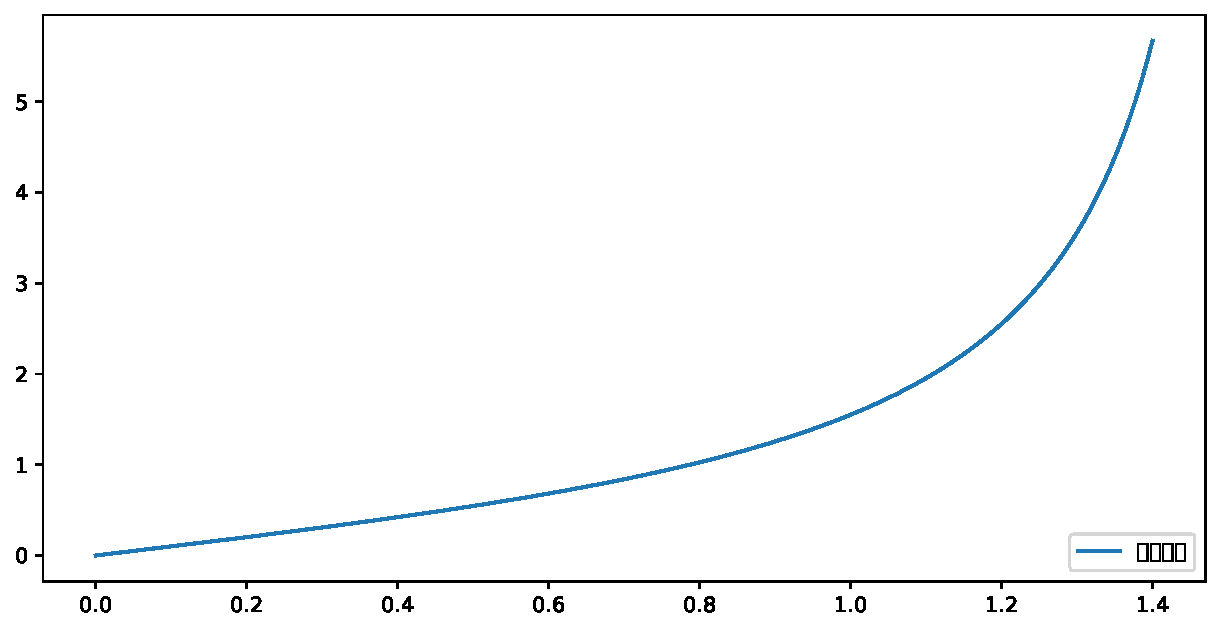
\includegraphics[width=\linewidth]{fig29.pdf}
\end{figure}

\paragraph{可视化代码}
~\\
\begin{minted}{python}
plt.figure(figsize=(10, 5))
plt.plot(t, y, label='欧拉方法')
plt.legend(loc='lower right')
plt.show()
\end{minted}

\subsubsection{题目1.3}

通过求题目1.1中欧拉方法的纵坐标平均值来估计平均感染个体数目。

编程求得平均感染数目为$22292.56481490718$。

\paragraph{代码}
~\\
\begin{minted}{python}
np.mean(y)
\end{minted}

\subsubsection{题目1.4}

通过使用曲线拟合题目1.1中的数据,并使用积分中值定理,估计平均感染个体的数目。

Logistic模型
$$f(x) = \frac{L}{1 + e^{ax + b}}$$

\begin{figure}[H]
	\centering
	\caption{欧拉方法与最小二乘拟合对比}
	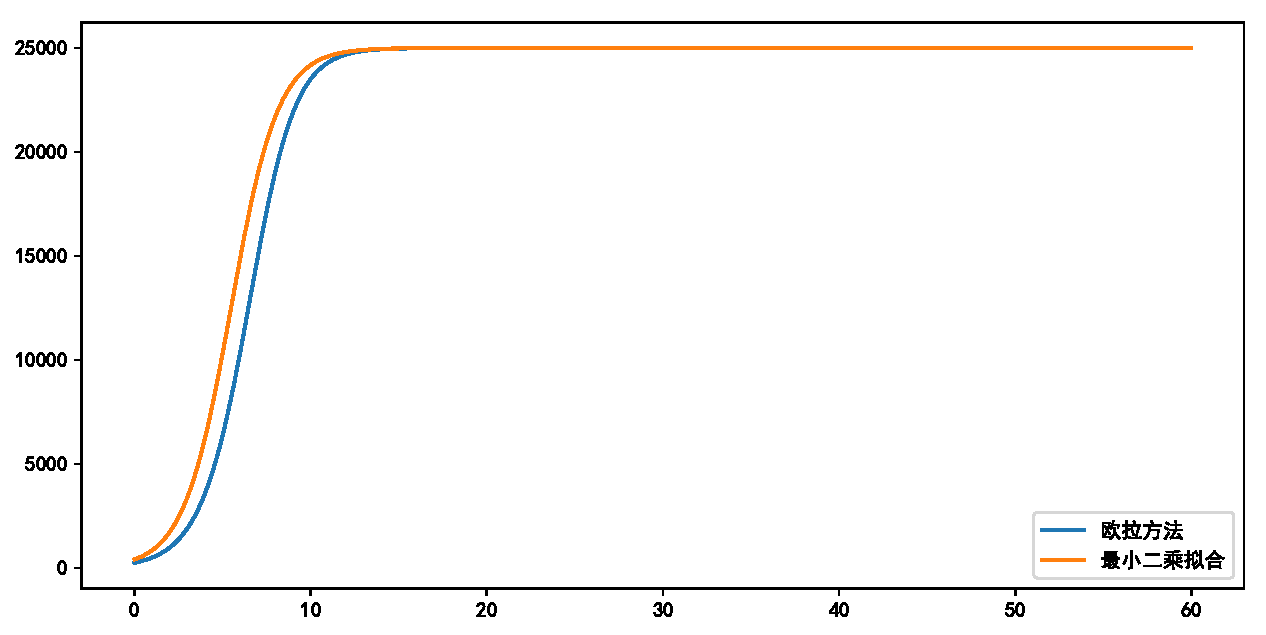
\includegraphics[width=\linewidth]{fig30.pdf}
\end{figure}

使用积分中值定理估计平均感染个体的数目为$22709.106862921362$。

\paragraph{代码}
~\\
\begin{minted}{python}
integrate.quad(lambda x: 25000.0 / (1 + np.exp(p(x))), 
               0, 60)[0] / 60
\end{minted}

\pagebreak

\subsection{题目2}

考虑一阶积分-常微分方程(intergro-ordinary differential equation) $$y'=1.3y-0.25y^2-0.0001y\int_0^ty(\tau)d\tau$$

\paragraph{常微分方程组解法}
~\\
给定一个常微分方程组:
$$\left\{
\begin{aligned}
\frac{dy_1}{dx} &= f_1\left(x,y_1,y_2,\cdots,y_n \right) \\
\frac{dy_2}{dx} &= f_2\left(x,y_1,y_2,\cdots,y_n \right) \\
&\vdots \\
\frac{dy_n}{dx} &= f_n\left(x,y_1,y_2,\cdots,y_n \right)
\end{aligned}
\right.$$

初始状态$y_0^{\left(0\right)}, y_2^{\left(0\right)}, \cdots, y_n^{\left(0\right)}$已知.令$$
\left\{
\begin{aligned}
K_{i}^{\left(1\right)} &= h * f_i\left(x^{\left(k\right)},y_1^{\left(k\right)},\cdots,y_n^{\left(k\right)}\right) \\
K_{i}^{\left(2\right)} &= h * f_i\left(x^{\left(k\right)} + \frac{h}{2}, y_1^{\left(k\right)} + \frac{1}{2}K_{1}^{\left(1\right)}, \cdots, y_n^{\left(k\right)} + \frac{1}{2}K_{n}^{\left(1\right)}\right) \\
K_{i}^{\left(3\right)} &= h * f_i\left(x^{\left(k\right)} + \frac{h}{2}, y_1^{\left(k\right)} + \frac{1}{2}K_{1}^{\left(2\right)}, \cdots, y_n^{\left(k\right)} + \frac{1}{2}K_{n}^{\left(2\right)}\right) \\
K_{i}^{\left(4\right)} &= h * f_i\left(x^{\left(k\right)} + h, y_1^{\left(k\right)} + K_{1}^{\left(3\right)}, \cdots, y_n^{\left(k\right)} + K_{n}^{\left(3\right)}\right) \\										
\end{aligned}
\right.$$

\paragraph{高阶微分方程数值解}
~\\
给定一个$n$阶微分方程, 且知道这个方程在某初始点处函数值和$1$到$n-1$阶导数值.求解方程:
$$y^{\left(n\right)} = f\left(x,y,y^{'},\cdots,y^{\left(n-1 \right)} \right)$$
令$y = y_1, y^{'} = y_2, y^{''} = y_3, \cdots, y^{\left(n-1\right)} = y_{n}$
可以转化为下面的形式:
$$\left\{
\begin{aligned}
y &= y_1 \\
\frac{dy_1}{dx} &= y_2 \\
\frac{dy_2}{dx} &= y_3 \\
&\vdots \\ 
\frac{dy_{n}}{dx} &= f\left(x,y,y_1,\cdots,y_{n}\right)
\end{aligned}
\right.$$

\pagebreak

\subsubsection{题目2.1}

在区间$[0,20]$上,用欧拉方法和$h=0.2,y(0)=250$以及梯形公式求方程的近似解。

\paragraph{分析}

欧拉方法的一般步长可以修改为
$$y_(k+1)=y_k+h(1.3y_k-0.25y_k^2-0.0001y_k\int_{0}^{t_k}y(\tau)d\tau)$$


如果梯形公式用于逼近积分,则该表达式为
$$y_(k+1)=y_k+h(1.3y_k-0.25y_k^2-0.0001y_k T_k (h))$$

其中$T_0 (h)=0$且
$T_k (h)=T_{k-1}(h)+\frac{h}{2} (y_{k-1}+y_k )$  其中$ k=0,1,…,99$

\paragraph{求解} 使用欧拉方法和梯形公式进行求解。

\begin{table}[H]
	\centering
	\caption{前9个近似解}
	\begin{tabular}{ll}
		\hline
		$t$      & $y$            \\ \hline
		0.000000 & 2.500000e+02   \\
		0.202020 & -2.810000e+03  \\
		0.404040 & -3.983600e+05  \\
		0.606061 & -7.935358e+09  \\
		0.808081 & -3.148621e+18  \\
		1.010101 & -4.957105e+35  \\
		1.212121 & -1.228694e+70  \\
		1.414141 & -7.548744e+138 \\
		1.616162 & -2.849290e+276 \\ \hline
	\end{tabular}
\end{table}

\paragraph{代码}
~\\
\begin{minted}{python}
h = 0.2
M = int(20 / h)
x = np.linspace(0, 20, M)
y = np.zeros(M)
t = np.zeros(M)
\end{minted}
\begin{minted}{python}
y[0] = 250
t[0] = 0
for k in range(M - 1):
    if k > 0:
        t[k] = t[k - 1] + h * (y[k - 1] + y[k]) / 2
    y[k + 1] = y[k] + h * (1.3 * y[k] 
                 - 0.25 * y[k] * y[k] - 0.0001 * y[k] * t[k])
display(pd.DataFrame(list(zip(x, y))[:10], columns=['$x$', '$y$']))
display(Math(r'\cdots'))
\end{minted}

\paragraph{迭代过程可视化}
~\\
\begin{figure}[H]
	\centering
	\caption{迭代过程可视化}
	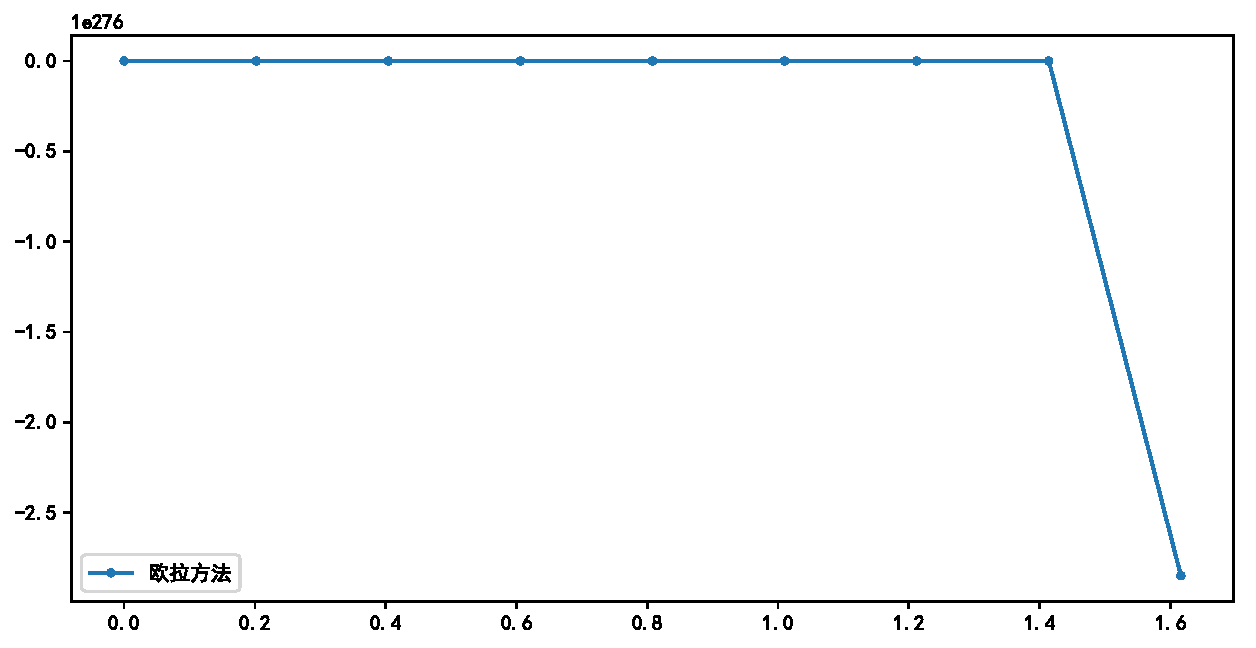
\includegraphics[width=\linewidth]{fig31.pdf}
\end{figure}

\subsubsection{题目2.2}

用初值$y(0)=200$和$y(0)=300$重复计算题目2.1的值。

\paragraph{求解} 使用欧拉方法和梯形公式进行求解。

\begin{table}[H]
	\centering
	\caption{$y(0)=200$和$y(0)=300$时前9个近似解}
	\begin{tabular}{ll}
		\hline
		\multicolumn{1}{c}{$t$} & \multicolumn{1}{c}{$y$} \\ \hline
		0.000000 & 2.000000e+02   \\
		0.202020 & -1.748000e+03  \\
		0.404040 & -1.549831e+05  \\
		0.606061 & -1.201232e+09  \\
		0.808081 & -7.215084e+16  \\
		1.010101 & -2.602976e+32  \\
		1.212121 & -3.387877e+63  \\
		1.414141 & -5.739085e+125 \\
		1.616162 & -1.646921e+250 \\ \hline
	\end{tabular}
\quad
	\begin{tabular}{ll}
		\hline
		\multicolumn{1}{c}{$t$} & \multicolumn{1}{c}{$y$} \\ \hline
		0.000000 & 3.000000e+02   \\
		0.202020 & -4.122000e+03  \\
		0.404040 & -8.547694e+05  \\
		0.606061 & -3.653409e+10  \\
		0.808081 & -6.673966e+19  \\
		1.010101 & -2.227180e+38  \\
		1.212121 & -2.480265e+75  \\
		1.414141 & -3.075980e+149 \\
		1.616162 & -4.731015e+297 \\ \hline
	\end{tabular}
\end{table}

\paragraph{迭代过程可视化}
~\\
\begin{figure}[H]
	\centering
	\caption{迭代过程可视化}
	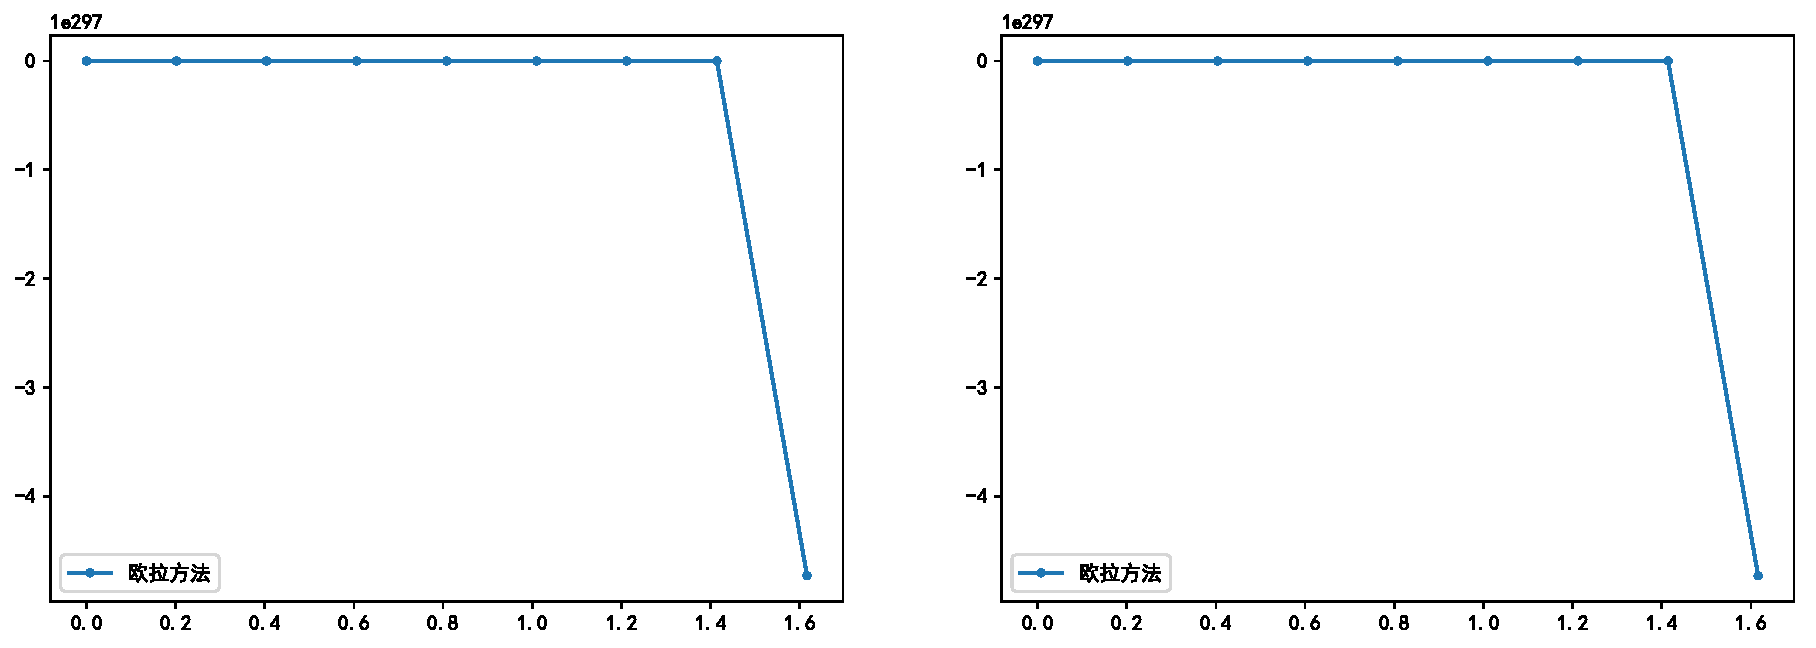
\includegraphics[width=\linewidth]{fig32.pdf}
\end{figure}

\subsubsection{题目2.3}

在同一坐标系下画出题目2.1和题目2.3的近似解,如下图所示。

\begin{figure}[H]
	\centering
	\caption{不同初值在同一坐标系下的对比图}
	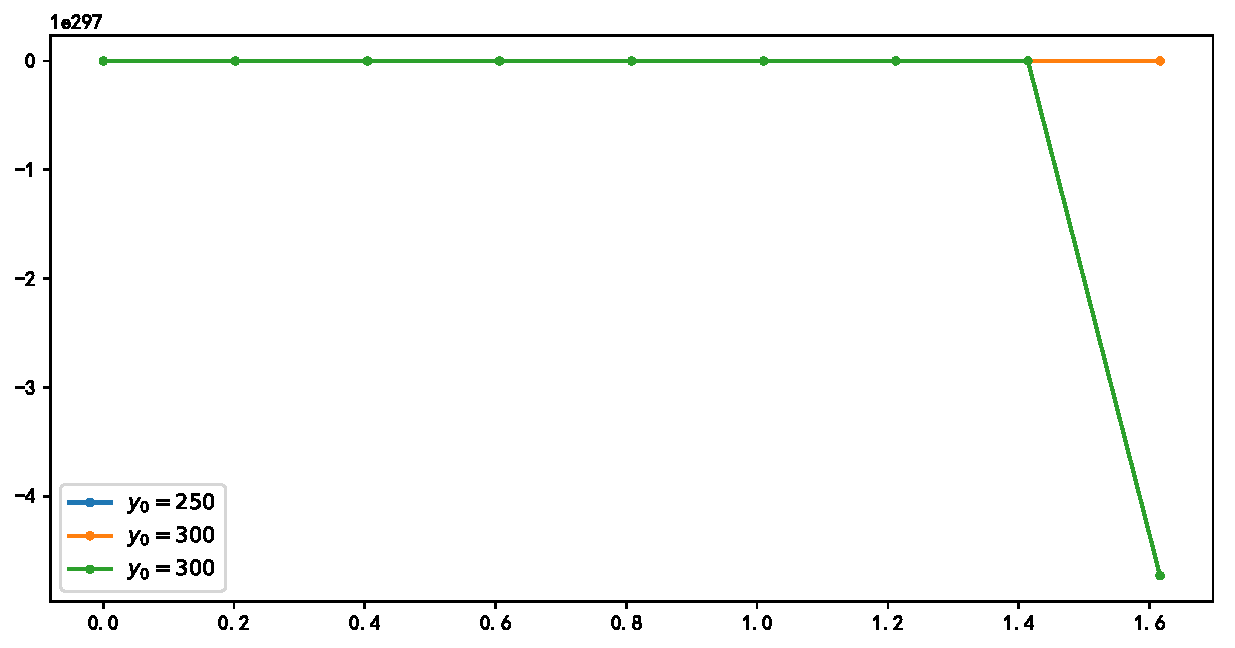
\includegraphics[width=\linewidth]{fig33.pdf}
\end{figure}

\subsection{题目3}

使用休恩方法求解微分方程
$$y'=3y+3t\qquad y(0)=1\qquad y(t)=\frac{4}{3}e^{3t}-t-\frac{1}{3}$$

\subsubsection{题目3.1}

令$h=0.1$,使程序执行20步,然后令$h=0.05$,使程序执行40步。

\begin{minted}{python}
def heun(f, a, b, ya, M):
    h = (b - a) / M
    T = np.linspace(a, b, M)
    Y = np.zeros(M)
    Y[0] = ya
    for j in range(M - 1):
        k1 = f(T[j], Y[j])
        k2 = f(T[j + 1], Y[j] + h * k1)
        Y[j + 1] = Y[j] + (h / 2) * (k1 + k2)
    return T, Y
\end{minted}

\subsubsection{题目3.2}

比较(a)中两个近似解与精确解$y(2)$。

\begin{table}[H]
	\centering
	\caption{$h=0.1$和$h=0.0.5$时近似解与解析解对比表}
	\begin{tabular}{lll}
		\hline
		\multicolumn{1}{c}{$t$} & \multicolumn{1}{c}{$\hat{y}$} & \multicolumn{1}{c}{$y$} \\ \hline
		0.000000                & 1.000000                      & 1.000000                \\
		0.105263                & 1.360789                      & 1.389859                \\
		0.210526                & 1.882367                      & 1.963577                \\
		0.315789                & 2.620205                      & 2.789429                \\
		0.421053                & 3.648912                      & 3.961043                \\
		0.526316                & 5.068840                      & 5.606815                \\
		0.631579                & 7.014958                      & 7.902818                \\
		0.736842                & 9.668802                      & 11.090512               \\
		0.842105                & 13.274539                     & 15.501017               \\ \hline
	\end{tabular}
	\quad
	\begin{tabular}{lll}
		\hline
		\multicolumn{1}{c}{$t$} & \multicolumn{1}{c}{$\hat{y}$} & \multicolumn{1}{c}{$y$} \\ \hline
		0.000000                & 1.000000                      & 1.000000                \\
		0.051282                & 1.165096                      & 1.170467                \\
		0.102564                & 1.365083                      & 1.377812                \\
		0.153846                & 1.605588                      & 1.628171                \\
		0.205128                & 1.893142                      & 1.928696                \\
		0.256410                & 2.235335                      & 2.287730                \\
		0.307692                & 2.640975                      & 2.715005                \\
		0.358974                & 3.120293                      & 3.221870                \\
		0.410256                & 3.685172                      & 3.821560                \\ \hline
	\end{tabular}
\end{table}

\paragraph{$h=0.1$和$h=0.0.5$时近似解与解析解对比图}
~\\
\begin{figure}[H]
	\centering
	\caption{$h=0.1$和$h=0.0.5$时近似解与解析解对比图}
	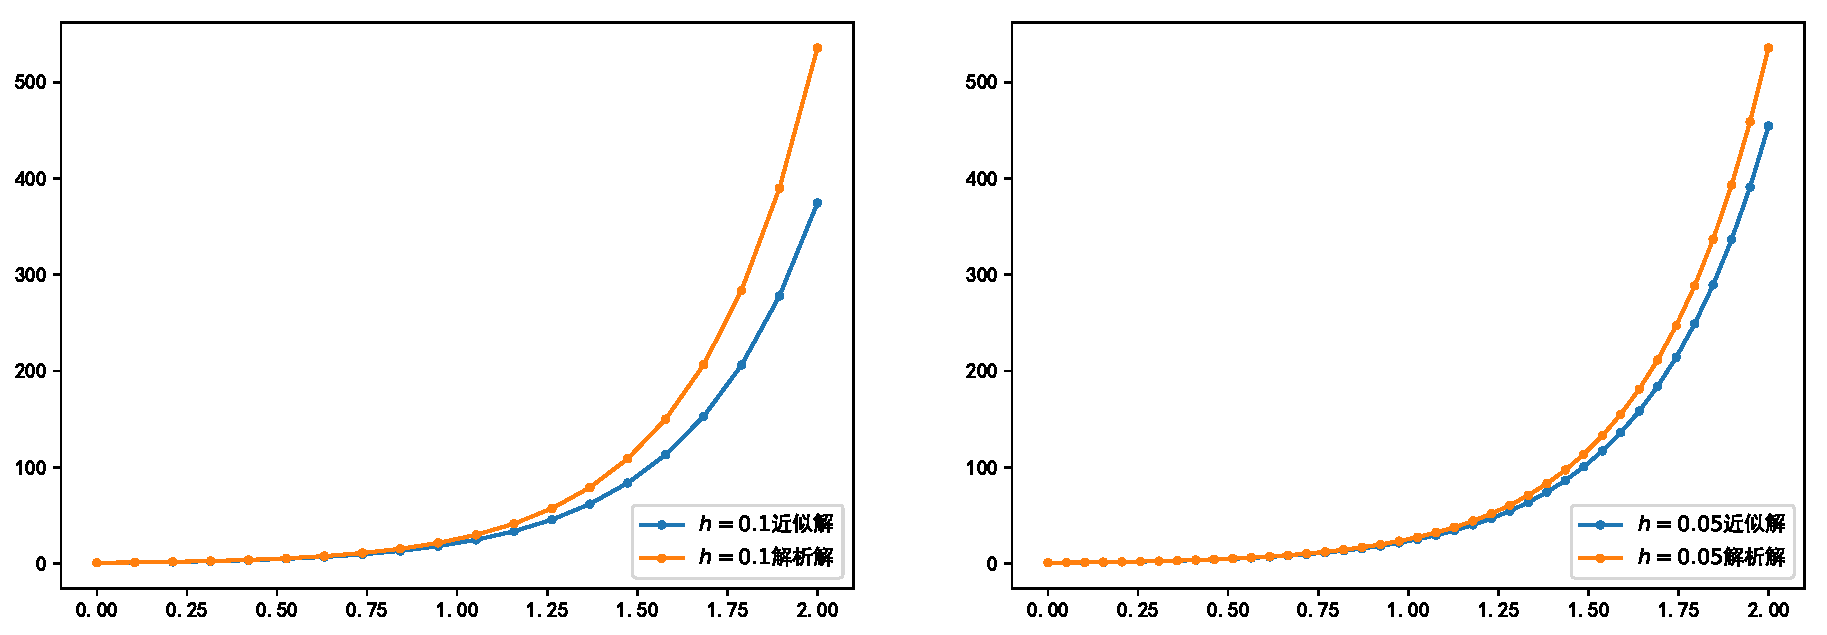
\includegraphics[width=\linewidth]{fig34.pdf}
\end{figure}

\subsubsection{题目3.3}

当h减半时,(a)中的最终全局误差是否和预期相符?

使用欧拉方法也有误差$O(h)$,和外面的$\frac{2}{h}$合在一起就是$O(h^2)$,所以总的误差就是$O(h^2)$。
所以如果步长变为原来的$\frac{1}{2}$误差应该变为原来的$\frac{1}{4}$

\subsubsection{题目3.4}

将两个近似解和精确解画在同一坐标系中。

\begin{figure}[H]
	\centering
	\caption{$h=0.1$和$h=0.0.5$时近似解与解析解对比图}
	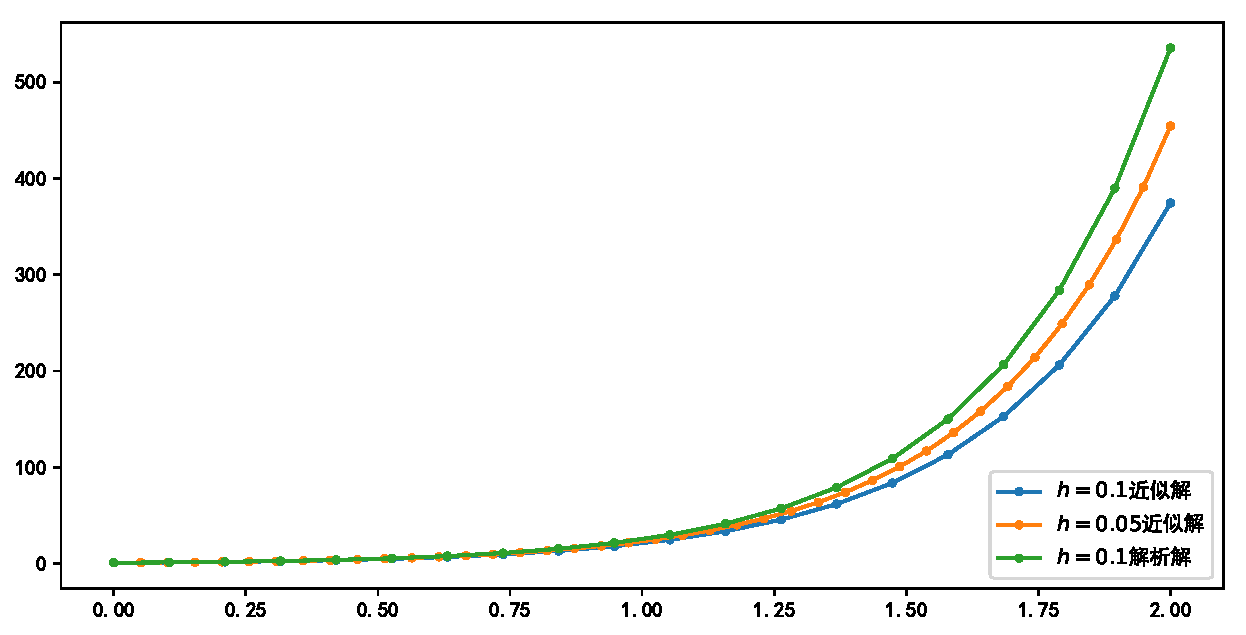
\includegraphics[width=\linewidth]{fig35.pdf}
\end{figure}

\subsection{题目4}

使用$N=4$的龙格-库塔方法求解微分方程
$$y'=3y+3t\qquad y(0)=1\qquad y(t)=\frac{4}{3}e^{3t}-t-\frac{1}{3}$$

\subsubsection{题目4.1}

令$h=0.1$,使程序执行20步,然后令$h=0.05$,使程序执行40步。

\begin{minted}{python}
def rk4(f, a, b, ya, M):
    h = (b - a) / M
    T = np.linspace(a, b, M)
    Y = np.zeros(M)
    Y[0] = ya
    for j in range(M - 1):
        k1 = h * f(T[j], Y[j])
        k2 = h * f(T[j] + h / 2, Y[j] + k1 / 2)
        k3 = h * f(T[j] + h / 2, Y[j] + k2 / 2)
        k4 = h * f(T[j] + h, Y[j] + k3)
        Y[j + 1] = Y[j] + (k1 + 2 * k2 + 2 * k3 + k4) / 6
    return T, Y
\end{minted}

\subsubsection{题目4.2}

比较(a)中两个近似解与精确解$y(2)$。

\begin{table}[H]
	\centering
	\caption{$h=0.1$和$h=0.0.5$时近似解与解析解对比表}
	\begin{tabular}{lll}
		\hline
		\multicolumn{1}{c}{$t$} & \multicolumn{1}{c}{$\hat{y}$} & \multicolumn{1}{c}{$y$} \\ \hline
		0.000000                & 1.000000                      & 1.000000                \\
		0.105263                & 1.360789                      & 1.389859                \\
		0.210526                & 1.882367                      & 1.963577                \\
		0.315789                & 2.620205                      & 2.789429                \\
		0.421053                & 3.648912                      & 3.961043                \\
		0.526316                & 5.068840                      & 5.606815                \\
		0.631579                & 7.014958                      & 7.902818                \\
		0.736842                & 9.668802                      & 11.090512               \\
		0.842105                & 13.274539                     & 15.501017               \\ \hline
	\end{tabular}
	\quad
	\begin{tabular}{lll}
		\hline
		\multicolumn{1}{c}{$t$} & \multicolumn{1}{c}{$\hat{y}$} & \multicolumn{1}{c}{$y$} \\ \hline
		0.000000                & 1.000000                      & 1.000000                \\
		0.051282                & 1.165096                      & 1.170467                \\
		0.102564                & 1.365083                      & 1.377812                \\
		0.153846                & 1.605588                      & 1.628171                \\
		0.205128                & 1.893142                      & 1.928696                \\
		0.256410                & 2.235335                      & 2.287730                \\
		0.307692                & 2.640975                      & 2.715005                \\
		0.358974                & 3.120293                      & 3.221870                \\
		0.410256                & 3.685172                      & 3.821560                \\ \hline
	\end{tabular}
\end{table}

\paragraph{$h=0.1$和$h=0.0.5$时近似解与解析解对比图}
~\\
\begin{figure}[H]
	\centering
	\caption{$h=0.1$和$h=0.0.5$时近似解与解析解对比图}
	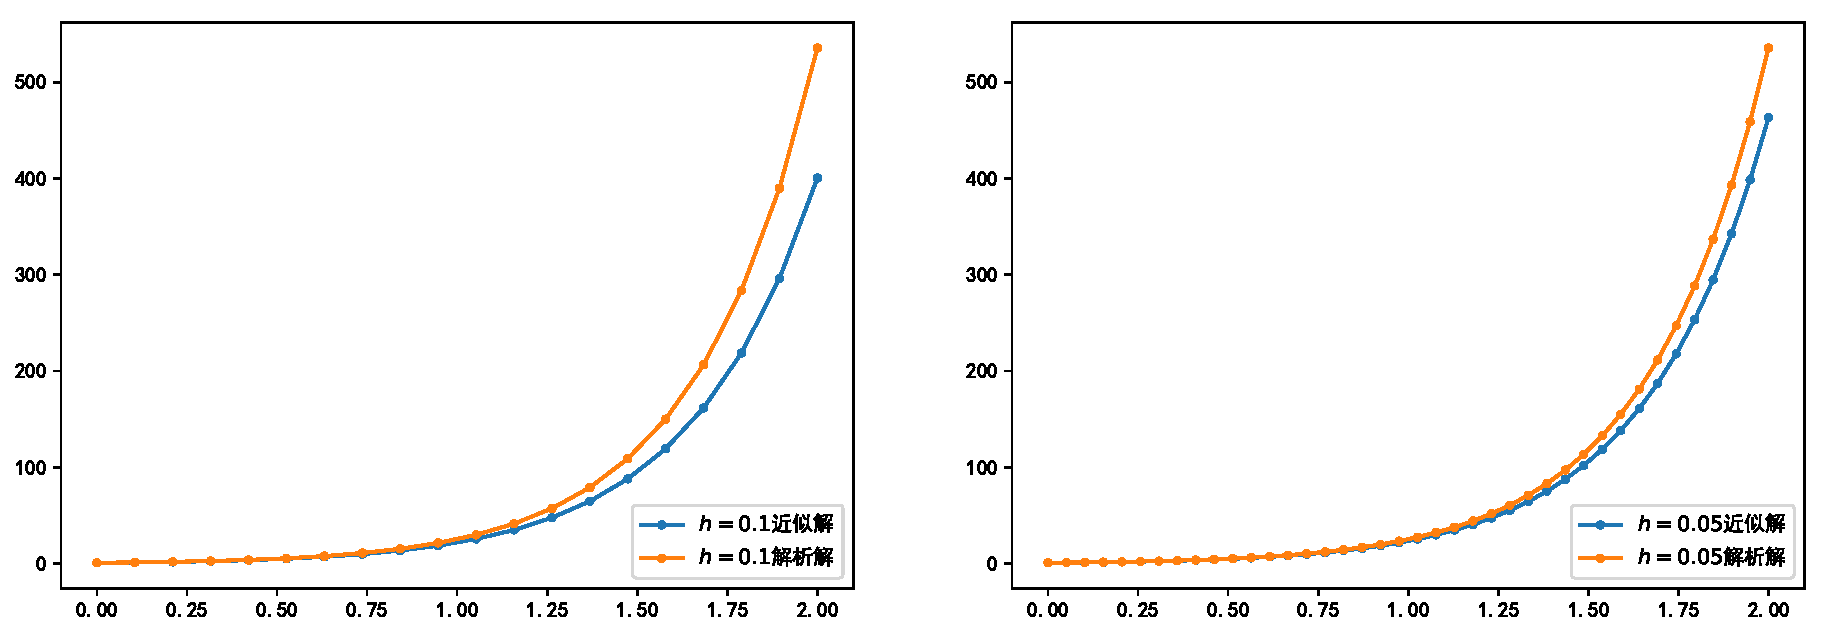
\includegraphics[width=\linewidth]{fig36.pdf}
\end{figure}


\subsubsection{题目4.3}

当h减半时,(a)中的最终全局误差是否和预期相符?

是的。

\subsubsection{题目4.4}

将两个近似解和精确解画在同一坐标系中。

\begin{figure}[H]
	\centering
	\caption{$h=0.1$和$h=0.0.5$时近似解与解析解对比图}
	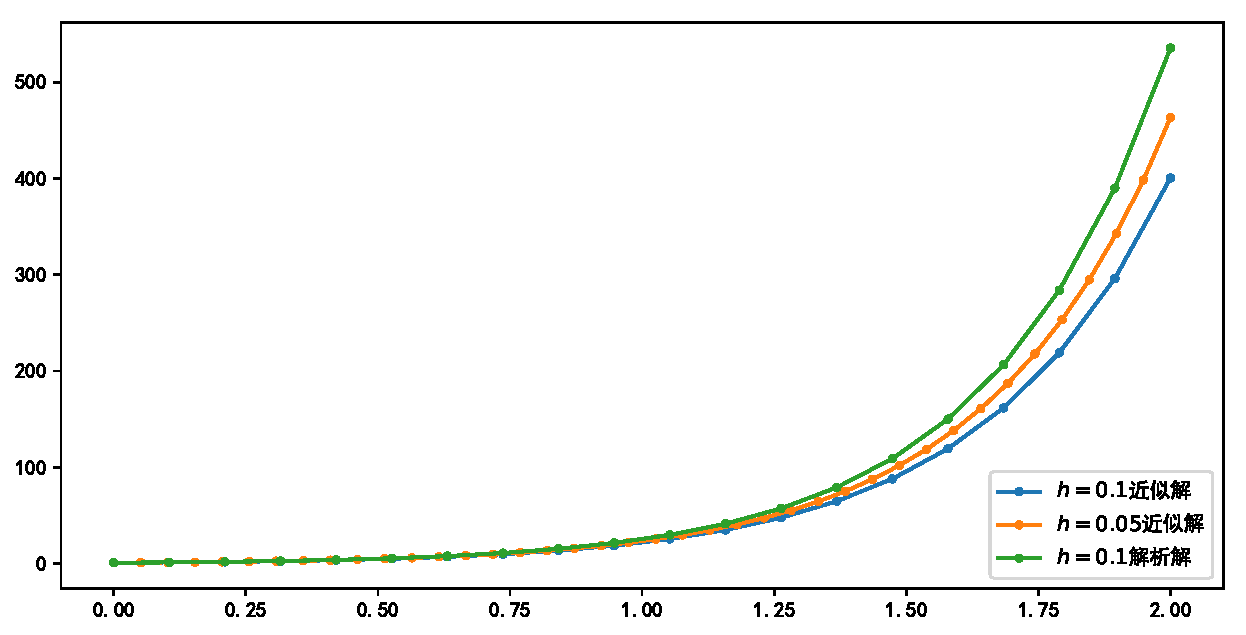
\includegraphics[width=\linewidth]{fig37.pdf}
\end{figure}